\chapter{Analisis dan Rancangan Jalur Komunikasi Sistem Simulasi}

Pada bab ini akan dibahas analisis permasalahan pada sistem simulasi yang sudah
ada. Setelah itu, akan dilakukan analisis terhadap solusi yang akan dibahas pada
juga pada bab ini. Lalu, akan dibahas perancangan perbaikan sistem simulasi.

\section{Analisis Masalah Sistem Simulasi}

Sistem simulasi yang ada sudah dapat menghubungkan server CARLA dengan server
NVIDIA Pegasus. Kedua server dihubungkan di sebuah jaringan menggunakan sebuah
layanan web. Layanan web ini memanfaatkan teknologi HTTP 1.1.

Solusi yang memanfaatkan layanan web dan HTTP ini merupakan \textit{bottleneck}
besar pada sistem simulasi. Kinerja yang diberikan pada arsitektur sekarang
sangat buruk. Dari 4000 transaksi per detik pada SILS, ketika menggunakan HILS
dan layanan web, turun menjadi 100-110 transaksi per detik. Kinerja buruk ini
mengakibatkan sistem simulasi terhambat pada jalur komunikasinya.

Selain itu, teknologi HTTP di bawah HTTP 2.0 juga tidak mendukung data
\textit{binary} dengan baik. Hal ini mengakibatkan data dari sensor membutuhkan
waktu dan \textit{resource} lebih untuk pemrosesannya.

Berdasarkan analisis masalah, dibutuhkan pembaruan pada sistem simulasi agar
memiliki kinerja yang lebih baik. Kinerja yang lebih baik ini bisa didapatkan
dengan mengubah metode komunikasi antara server CARLA dan server Pegasus. Selain
itu, jalur komunikasi juga harus mendukung pengiriman data \textit{binary}.
Selain cepat dan mendukung \textit{binary}, jalur komunikasi tentu saja harus
reliabel agar tidak ada data yang hilang.

\section{Analisis Solusi}

Solusi yang dapat diberikan untuk masalah pada sistem simulasi adalah pembaruan
pada arsitektur sistem solusi dan mengganti metode komunikasi yang digunakan.
Pembaruan pada arsitektur akan menghilangkan \textit{middleware} layanan web di
antara server CARLA dengan server NVIDIA Pegasus. Lalu, metode komunikasi yang
akan digunakan harus dapat mendukung kebutuhan kinerja dan pengiriman data
\textit{binary}.

Metode komunikasi yang dapat digunakan ada beberapa pilihan. Metode-metode
tersebut adalah ZeroMQ, gRPC, dan ROS. ZeroMQ dipilih karena berjalan di atas
TCP yang artinya akan mendukung data \textit{binary}. Selain itu, ZeroMQ
mendukung berbagai skema komunikasi: \textit{pub/sub},
\textit{request/response}, dan \textit{push/pull}. Metode gRPC adalah
peningkatan dari protokol RPC yang menggunakan HTTP 2.0 sehingga memiliki
kinerja yang baik. HTTP 2.0 juga mendukung pengiriman data dalam bentuk
\textit{binary}.  Selain itu, gRPC mendukung \textit{data streaming} sehingga
cocok digunakan untuk kebutuhan pengiriman data dari sensor. Metode terakhir
adalah menggunakan ROS. ROS adalah sekumpulan kakas yang sering digunakan pada
lingkungan IoT. Selain itu pada percobaan sebelumnya
\parencite{brogle_CarlaHILS}, ROS sudah dibuktikan sebagai salah satu alternatif
metode komunikasi yang baik untuk sistem simulasi HILS. ROS sendiri mendukung
skema komunikasi \textit{pub/sub} dan \textit{request/response}.

Dari ketiga metode solusi tersebut akan dipilih yang memiliki kinerja paling
baik melalui beberapa percobaan. Percobaan ini akan dilakukan selama pembuatan
jalur komunikasi pada sistem simulasi HILS.

Selain pemilihan metode komunikasi, akan dilakukan pembaruan terhadap arsitektur
sistem simulasi. Layanan web akan dihilangkan sehingga server CARLA akan
berkomunikasi langsung dengan server Pegasus. Hal ini berpotensi mengakibatkan
berkurangnya latensi ketika terjadi komunikasi antara server CARLA dengan server
Pegasus.

\section{Rancangan Pembuatan Jalur Komunikasi Sistem Simulasi}

Proses perancangan pembuatan jalur komunikasi sistem simulasi seperti diagram
alir pada gambar \ref{chapter-3-perancangan}. Perancangan diawali dengan
mengubah arsitektur sistem simulasi, setelah itu menambahkan \textit{monitoring}
sistem simulasi, lalu menganalisis data \textit{monitoring} untuk menentukan
metode komunikasi terbaik. Desain arsitektur baru untuk sistem simulasi dapat
dilihat pada lampiran \ref{appendix-arsitektur-baru}. Lalu, algoritma sistem
simulasi dapat dilihat pada lampiran \ref{appendix-algoritma-monitoring}.

\begin{center}
	\begin{figure}[ht]
		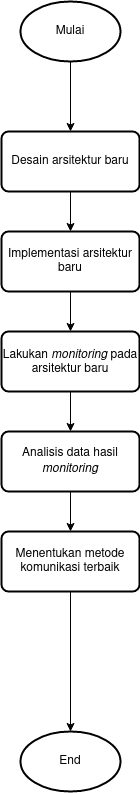
\includegraphics[height=0.6\textheight]{resources/chapter-3/flowchart-perancangan.png}
		\caption{Diagram Alir Perancangan Solusi}
		\label{chapter-3-perancangan}
	\end{figure}
\end{center}